\documentclass[a4paper,10pt]{article}
\usepackage{float}
\usepackage{graphicx}
\usepackage[ansinew]{inputenc}
\usepackage[spanish]{babel}
\usepackage{listings}
\usepackage{hyperref}
\usepackage{enumitem}
\inputencoding{latin1}
\graphicspath{/imagenes,/Casos de prueba}

\title{		\textbf{Trabajo Pr\'{a}ctico 0: \\
			Infraestructura b\'{a}sica
			}}

\author{	Fabrizio Cozza, \textit{Padr\'{o}n Nro. 97.402}                     \\
            \texttt{ fabrizio.cozza@gmail.com }                                              \\[2.5ex]
            Kevin Cajachu\'{a}n, \textit{Padr\'{o}n Nro. 98.725}                     \\
            \texttt{ kevincajachuan@hotmail.com }                                              \\[2.5ex]
            Luciano Giannotti, \textit{Padr\'{o}n Nro. 97.215}                     \\
            \texttt{luciano\_giannotti@hotmail.com.ar}                                              \\[3.5ex]
	 \newline
            \normalsize{1er. Cuatrimestre de 2018}                                      \\
            \normalsize{66.20 Organizaci\'{o}n de Computadoras  $-$ Pr\'{a}ctica Viernes}  \\
            \normalsize{Facultad de Ingenier\'{i}a, Universidad de Buenos Aires}            \\
       }
\date{}


\begin{document}
\maketitle
\thispagestyle{empty}   % quita el n�mero en la primer p�gina
\newpage

\section{Objetivos}

Este Trabajo Pr\'{a}ctico tiene el fin de ayudarnos a familiarizarnos con las herramientas de software que utilizaremos posteriormente en otros trabajos, como es el emulador \textbf{gxemul} para correr programas sobre una maquina MIPS con el Sitema Operativo NetBSD.


\section{Programa}

El software de este trabajo esta escrito en lenguaje C y permite dibujar \textbf{Julia Sets} o \textbf{Conjuntos de Julia} segun los par\'{a}metros que le pasamos por l\'{i}nea de comando.
Estos parámetros son la region del plano complejo: delimitada por un centro, un ancho y un alto; una semilla que afectara el calculo para c\'{a}da pixel; la resoluci\'{o}n y la salida ya sea por pantalla o por archivo.
El formato a usar es  PGM o \textit{portable gray format}, que resulta \'{u}til para describir im\'{a}genes digitales en escala de grises.


\section{Implementaci\'{o}n}

Una vez recibidos los par\'{a}metros, para dibujar el Julia Set el programa obtiene de cada p\'{i}xel de la ventana a un punto en el plano complejo.
A ese punto se lo eleva al cuadrado y le suma la semilla mencionada en la secci\'{o}n anterior. Esto se repite hasta que el valor absoluto del resultado sea menor a 2, en cuyo caso se toma la cantidad de iteraciones y se imprime en el archivo PGM, representando el nivel de blanco de ese pi\'{i}xel.


\section{C\'{o}digo C}

En esta secci\'{o}n colocaremos el ci\'{o}digo fuente del programa en lenguaje C.

\lstinputlisting[basicstyle=\ttfamily\scriptsize]{main.c}

\newpage

\section{Pruebas}

Para las pruebas compilamos el programa con gcc de la siguiente manera:

\begin{lstlisting}[frame=single]
$gcc main.c -o tp0
\end{lstlisting}
Luego corremos el archivo \textbf{test.sh}.
Ya que las pruebas son sobre las imágenes, las vamos a realizar a ojo comparandolas con las del enunciado y con las obtenidas en un generador online (\url{http://usefuljs.net/fractals/}).\\

Cabe destacar que las imagenes del generador tienen mayor rango dinamico que las del enunciado y nosotros decidimos generarlas como en \'{e}ste \'{u}ltimo.

Las imagenes obtenidas por nuestro trabajo se encuentran tambi\'{e}n en formato PNG en la subcarpeta \textit{imagenes}.
A su vez las imagenes del generador online se encuentran en \textit{Casos de prueba}.

\subsection{Caso con los valores por defecto}
Se obtiene una imagen como la primera figura del enunciado:

\begin{lstlisting}[frame=single]
$./tp0 -o uno.pgm
\end{lstlisting}

\begin{figure}[H]
\begin{center}
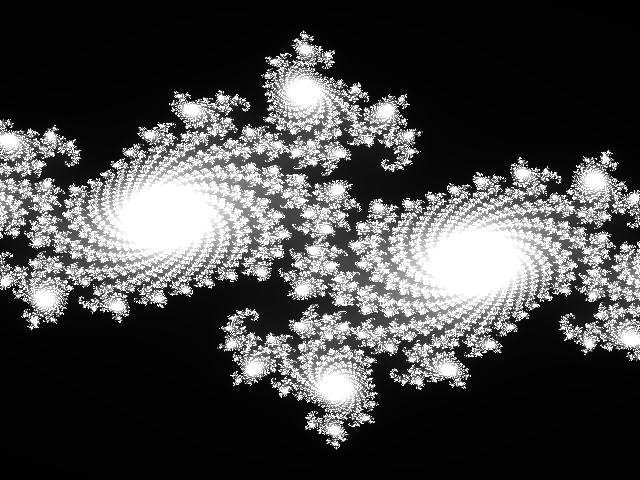
\includegraphics[width=0.5\textwidth]{imagenes/uno.png}
\caption{} \label{uno}
\end{center}
\end{figure}

\newpage

\subsection{Caso de imagen con zoom y otro centro}
Se obtiene una imagen como la segunda figura del enunciado:

\begin{lstlisting}[frame=single]
$ ./tp0 -c 0.282-0.007i -w 0.005 -H 0.005 -o dos.pgm
\end{lstlisting}

\begin{figure}[H]
\begin{center}
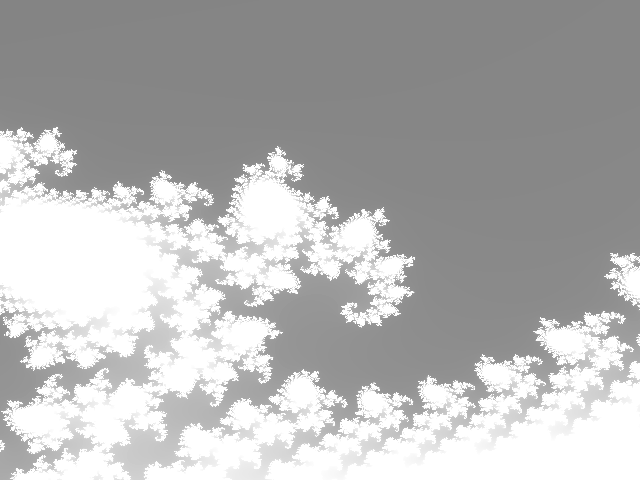
\includegraphics[width=0.5\textwidth]{imagenes/dos.png}
\caption{} \label{dos}
\end{center}
\end{figure}

\subsection{Caso de imagen con ancho 1 y centro 1}
Se obtiene una imagen como la primera del enunciado pero con un zoom x2 aplicado:

\begin{lstlisting}[frame=single]
$ ./tp0 -w 1 -H 1 -o tres.pgm
\end{lstlisting}

\begin{figure}[H]
\begin{center}
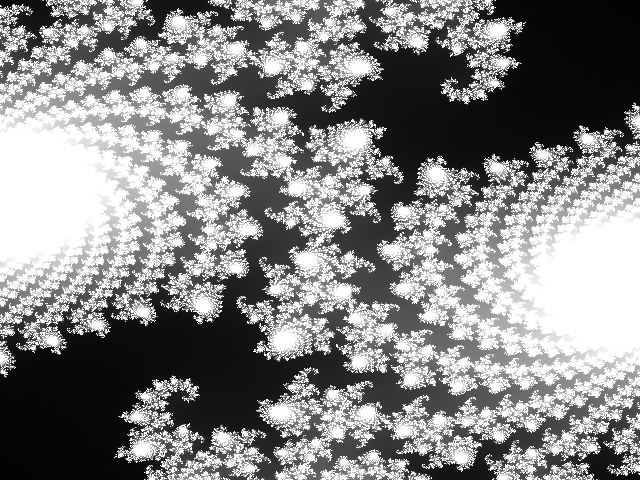
\includegraphics[width=0.5\textwidth]{imagenes/tres.png}
\caption{} \label{tres}
\end{center}
\end{figure}

\newpage

\subsection{Caso de imagen muy chica}

Imprimimos una imagen de 8x6 para que se puedan notar claramente los pixeles en la pantalla.

\begin{lstlisting}[frame=single]
$ ./tp0 -r 8x6 -o cuatro.pgm
\end{lstlisting}

\begin{figure}[H]
\begin{center}

\includegraphics[width=0.5\textwidth]{imagenes/cuatro.png}
\caption{} \label{cuatro}
\end{center}
\end{figure}

\subsection{Caso de imagen con otra semilla}

Esta imagen usa una semilla con sus dos componentes negativas y la imaginaria mucho mas grande que la real.
\begin{lstlisting}[frame=single]
$ ./tp0 -s -0.157-1.041i -o cinco.pgm
\end{lstlisting}

\begin{figure}[H]
\begin{center}
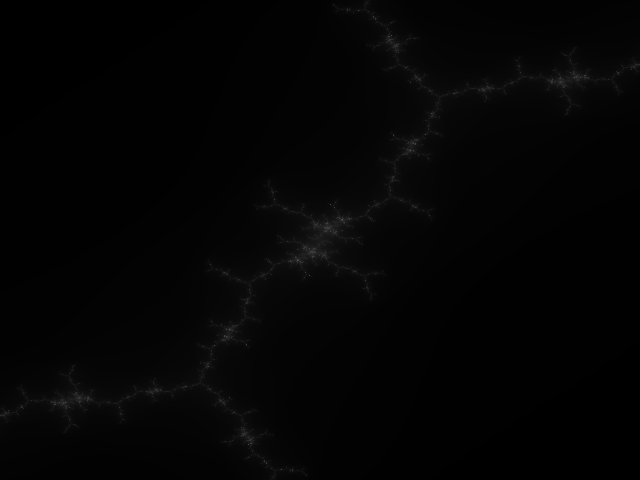
\includegraphics[width=0.5\textwidth]{imagenes/cinco.png}
\caption{} \label{cinco}
\end{center}
\end{figure}

\newpage

\subsection{Caso de imagen muy angosta}
En este caso cambiamos la resolucion para obtener una imagen de un pixel
de alto y 800 de ancho. Es dicil observarla en el informe por lo que decidimos
no colocarla. Sin embargo el archivo se encuentra en la misma carpeta del TP con el nombre \textit{seis.pgm}.

\begin{lstlisting}[frame=single]
$ ./tp0 -r 800x1 -o seis.pgm
\end{lstlisting}

\section{C\'{o}digo S}

En esta secci\'{o}n colocaremos el ci\'{o}digo assembly MIPS generado por NetBSD.

\lstinputlisting[basicstyle=\ttfamily\scriptsize]{main.s}

\section{Bibliograf\'{i}a}
\begin{enumerate}
\item GXemul. \\ http://gavare.se/gxemul/.
\item The NetBSD project. \\
	http://www.netbsd.org/.
\item http://es.wikipedia.org/wiki/Conjunto\_de\_Julia (Wikipedia).
\item PGM format specification.\\
	http://netpbm.sourceforge.net/doc/pgm.html.
\item Generador de fractales. \\
	http://usefuljs.net/fractals/
\item GIMP. \\
	https://www.gimp.org/
\end{enumerate}

\end{document}
